\documentclass[a4paper, 10pt]{article}
\usepackage{comment} % enables the use of multi-line comments (\ifx \fi) 
\usepackage{lipsum} %This package just generates Lorem Ipsum filler text. 
\usepackage{fullpage} % changes the margin
\usepackage{graphicx}
\usepackage{xcolor}

\begin{document}
%Header-Make sure you update this information!!!!
\noindent
\large\textbf{Middleware Project - IoT} \hfill \textbf{Marco Bacis} 873199 \\
Prof. Guinea \hfill \textbf{Daniele Cattaneo} 874757 \\
Prof. Mottola

\section*{Problem Statement}

The goal of the project is to develop an IPv6-based presence detection system using MQTT, in which every person is equipped with a wireless sensor, and every room has a static wireless device working as IPv6 border-router.
The mobile device detects the user movements and, when the user is stationary, starts sending MQTT messages containing the client ID on a topic which depends on the room.
The device should do everything possible to minimize energy consumption while the user is moving.
Finally, the parameters for the movement threshold (T), the acceleration reading period while the used is motionless (G), and other relevant parameters, should be configurable through the \texttt{project-conf.h} file.

\section*{Implementation}

\subsection*{Sensor Finite State Machine}

\begin{figure}[h]
\centering
    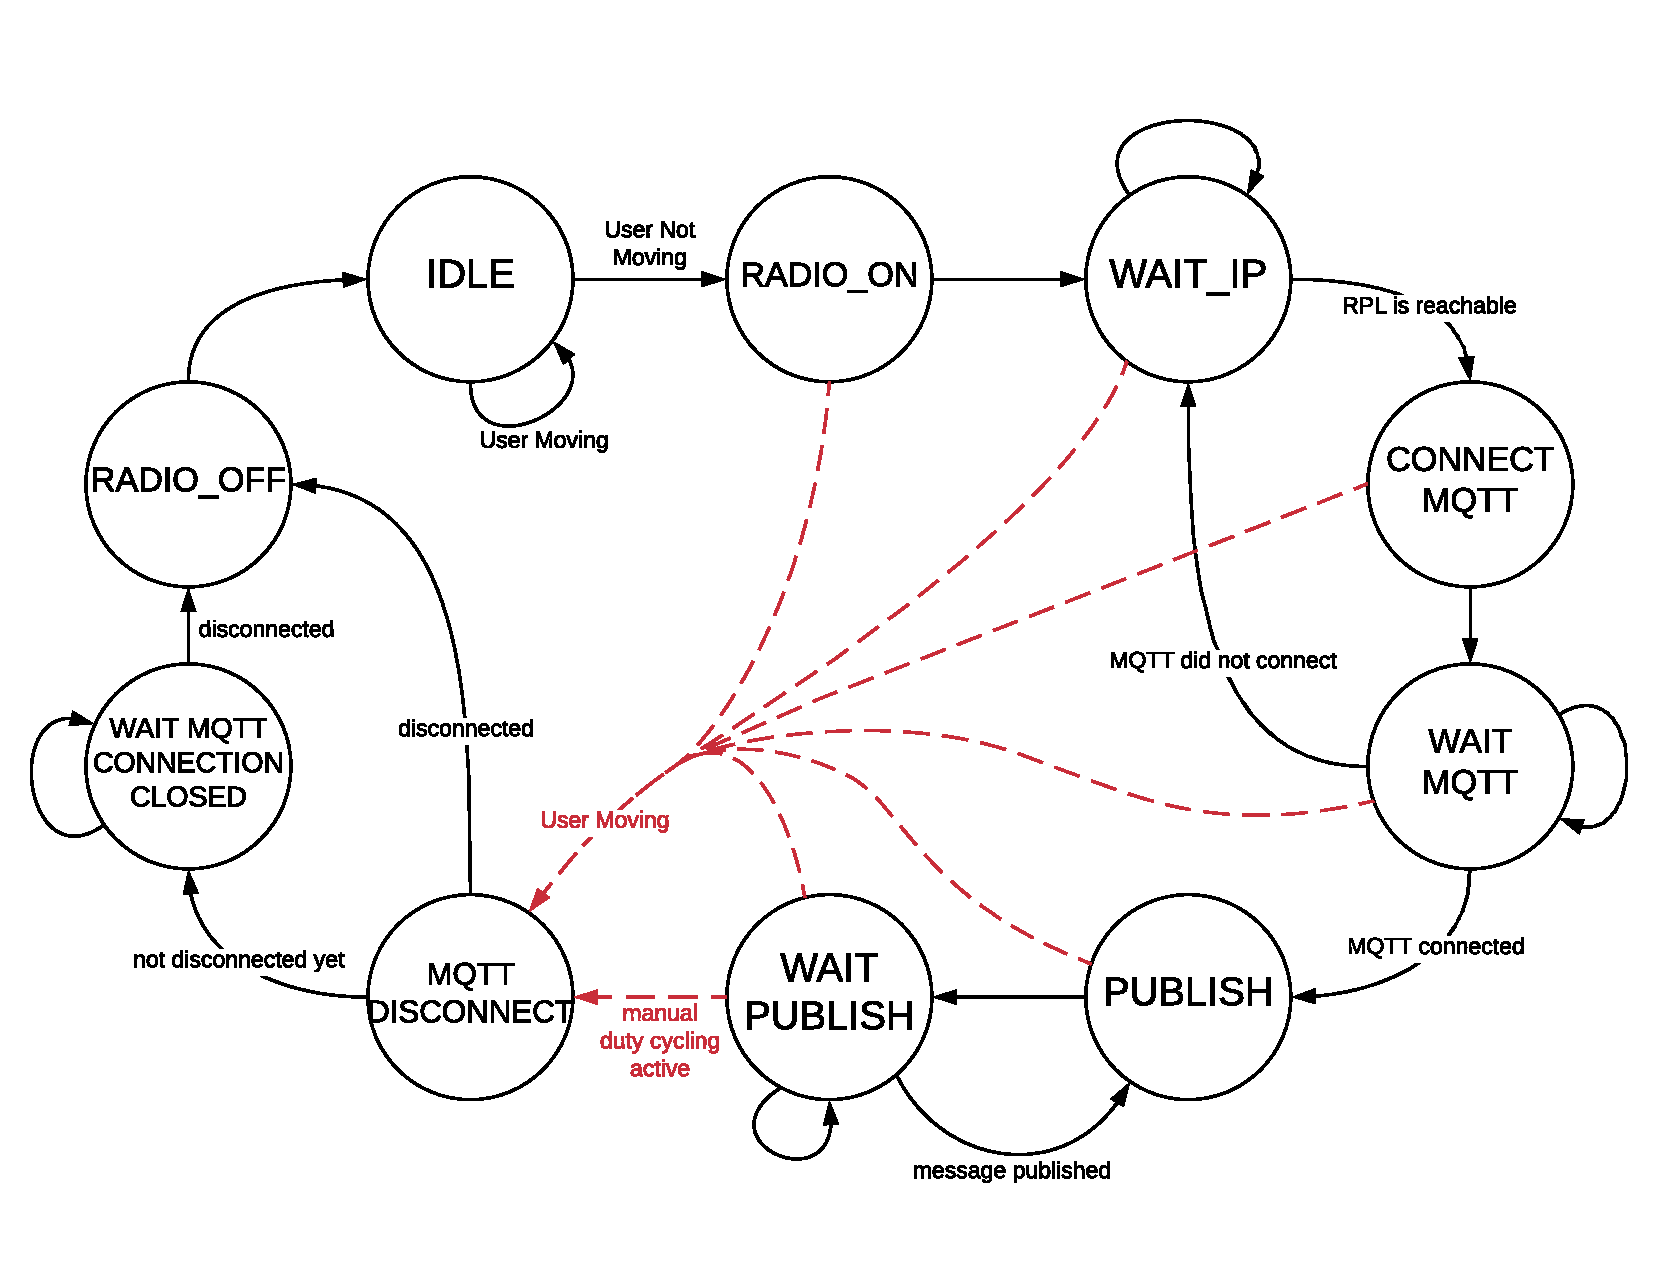
\includegraphics[width=\linewidth]{images/fsm.pdf}
    \caption{Finite State Machine responsible for the radio/MQTT connection and message publishing.}
    \label{fig:sensor_fsm}
\end{figure}

The main thread (\texttt{client\_process}) integrates a Finite State Machine (FSM) to manage the MQTT connection based on the reachability of a IP network and the user movements.
The FSM process is event-driven (being a Contiki protothread), but it also has a default timer of one second used when polling is needed (for example during connections).
The FSM can be seen in Figure~\ref{fig:sensor_fsm}, which highlights the states and relevant transitions.

The \texttt{IDLE} state is the source and sink state. In this state, the sensor doesn't perform any action apart from waiting for the user to stop moving.

When the user stops moving, the sensor turns the radio on and, when a network connection is established, it connects to an MQTT broker whose IP and port is configurable in \texttt{project-conf.h}.
After that, an MQTT message is published every \texttt{K} seconds on a topic whose last level corresponds to the IP address of the border router (which acts as room id). The exact name of the topic is configurable.
The contents of the message consists of a JSON dictionary with 6 key-value pairs: \texttt{client\_id}, \texttt{seq\_number}, \texttt{last\_accel}, \texttt{current\_rssi}, \texttt{current\_dbm\_power}, and \texttt{uptime}.

When the user starts moving (detected by the movement monitor process), the state is changed to \texttt{MQTT\_DISCONNECT} and the disconnection phase is performed.

If the connection is lost (either MQTT or RPL not reachable) and the user is not moving, the connection phase is attempted again by changing state to \texttt{WAIT\_IP}.

\subsection*{Parameters Estimation}

\begin{figure}[h]
\centering
    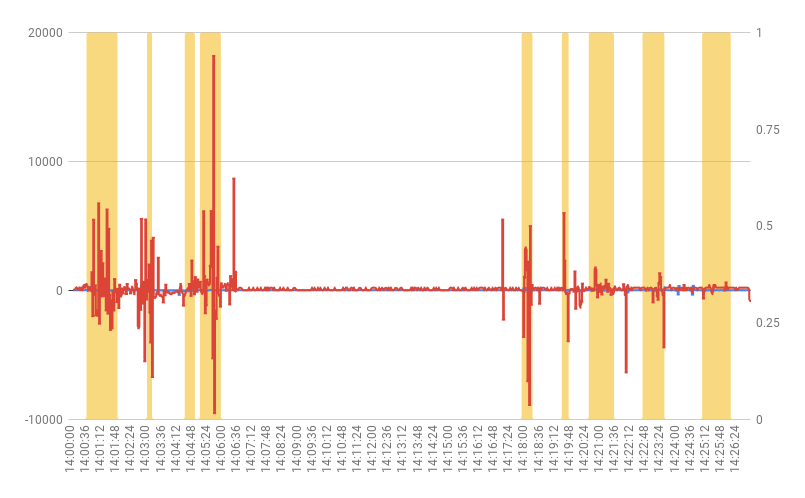
\includegraphics[width=0.7\linewidth]{images/accel_chart.png}
    \caption{Gathered movement data (modulus - $|\vec{g}|$) with movement periods highlighted.}
    \label{fig:accel_data}
\end{figure}

Two parameters were estimated: T (movement threshold) and G (movement read timeout while not moving).

For both parameters, real data were collected using the SensorTag board, and then analyzed in order to get a fair estimate.
The data was collected while a user moved in his house with the SensorTag attached doing menial tasks.
The accelerator data and the detected movement is shown in Figure~\ref{fig:accel_data}.

The movement threshold T is applied to the square of the modulus of the acceleration, minus the modulus of the gravity acceleration, in absolute value. It was estimated by trying to match the detected movements with the real ones. We estimated $T = 1000$ roughly. Also, a second threshold (\texttt{T\_DMOD}) is applied to the difference between the current and previous moduli in absolute value, and has been set to half the general threshold.

The reading timeout G is an environment and use-case dependent factor -- it depends on the place in which the system is deployed and which activities the users are performing.
The measure of G impacts on the resolution of the system (not counting disconnections when moving too far from the router), so it must be a lower bound based on some experimental data gathered from the environment.
In our case, we used a \emph{smooth} representation of the acceleration data to obtain the movements (without counting small movements in the same room).
The average movement lasted 42 seconds with a $23,29$ standard deviation, a minimum time of 12 seconds and maximum of 74 seconds.
As a tradeoff between resolution and energy consumption we decided to estimate G as $average - standard deviation$ from the test data, meaning $G = 19$ seconds.
In this way, G lasts less than $84,1$\% of the movement periods, and at least one acceleration measure is done in longer periods.

\subsection*{Energy Consumption minimization}
In order to reduce the energy consumption of the device, two features were added to the client code, one for acceleration readings and the other for the network connection.

As for the data movement reading, the movement sensor (MPU 9250) is activated only when necessary (only while reading). 

The network connections impacts heavily on the client energy consumption. To reduce this, two options can be configured in the client code apart from the default CSMA mode: TSCH, or manual CSMA duty cycling.

In default CSMA mode, the radio is turned off when the user is moving, and it is turned on when the user is not moving.

In TSCH mode, the duty cycling mechanism is handled transparently underneath RPL, meaning that user moving or not moving does not imply client connected or not.

In manual CSMA duty cycling mode, the radio is turned on only for the duration of time needed to connect to the MQTT broker and send a single message, then it is turned off immediately. To avoid continual connections and disconnections for small values of K (which increase power consumption), the time needed to send a message is not counted against the publishing period K.

Table~\ref{table:energest} shows energy consumption data for each of the modes, collected using Energest. Each test had a duration of 10 minutes.
It can be seen that manual duty cycling over CSMA (DutyCycling) has the lowest possible power draw while the user is moving, and is suitably low also while motionless, as it drastically reduces the CPU activity with respect to the default CSMA mode.
On the other hand, TSCH has a lower energy consumption while motionless, but it keeps the CPU active for longer periods to check the radio state.


\begin{table}[!htb]
\begin{tabular}{ll|ccc|cc|c}
& & \multicolumn{3}{c|}{ \textbf{CPU Mode (s)} } & \multicolumn{2}{c|}{ \textbf{Radio (s)} } & \\
\textbf{MAC} & \textbf{Action} & \textbf{Active} & \textbf{Sleep} & \textbf{Deep Sleep} & \textbf{Listening} & \textbf{Transmit} & \textbf{Energy (J)} \\
CSMA & Motionless & 1 & 2 & 596 & 0 & 0 & 0.05 \\
CSMA & Moving & 13 & 581 & 5 & 592 & 2 & 11.59 \\
CSMA & DutyCycling & 13 & 273 & 312 & 280 & 3 & 5.58 \\
TSCH & Moving & 174 & 24 & 401 & 163 & 0 & 8.39 \\
TSCH & Standing & 157 & 28 & 414 & 53 & 3 & 2.43 \\
TSCH & StandNoLed & 209 & 22 & 367 & 107 & 2 & 3.81 \\
\end{tabular}
\caption{Energest test data}
\label{table:energest}
\end{table}

%\section*{Attachments}
%Make sure to change these
%Lab Notes, HelloWorld.ic, FooBar.ic
%\fi %comment me out


\end{document}
